\section{Experiments}

\subsection{Question 1}
The score of the alignment between bos\_taurus, canis\_lupus, and gallus\_gallus is 790, with the alignment being: 

\begin{verbatim}
atggatttatctgcggatcatgttgaagaagtacaaaatgtcctcaatgctatgca-gaaaatcttag--agtgtccaat-atgtctggagttgatcaaagag-cct-gtctctacaaagtgtga-cca-ca-tattttgcaaattttg-tatgctgaa-ac-ttctcaacca-gaagaaagggccttcacaatgtcc--tttgtgtaagaatga-

atggatttatctgcggatcgtgttgaagaagtacaaaatgttcttaatgctatgca-gaaaatcttag--agtgtccaat-atgtctggagttgatcaaagag-cct-gtttctacaaagtgtga-tca-ca-tattttgcaaattttg-tatgctgaa-ac-ttctcaacca-gaggaaggggccttcacagtgtcc--tttgtgtaagaacga-

gcgaa---atgta-aca-cg-gtagaggtgat-cggggtg-cgtt-atac-gtgcgtggtgacctcggtcggtgt-tgacggtgcctggggttcctcagagtgttttggggtctgaaggatg-gacttgtcagtg-attgccattggagacgtgcaaaatgtgctttcagccatgcagaa-gaa-ctt-ggagtgtccagtctgtttagatgtgat
\end{verbatim}

\subsection{Question 2}
The score by sp\_approx is 4688, and the center string is sequence 4, homo\_sapiens.
We computed the score for the various permutations of the remaining 4 sequences, and they all score the same, 4688. 

This is because we are very conservative with the way we add sequences, we do not collapse, and therefore the score will always remain the same, no matter the order of the sequences. 

\subsection{Question 3}
\begin{center}
    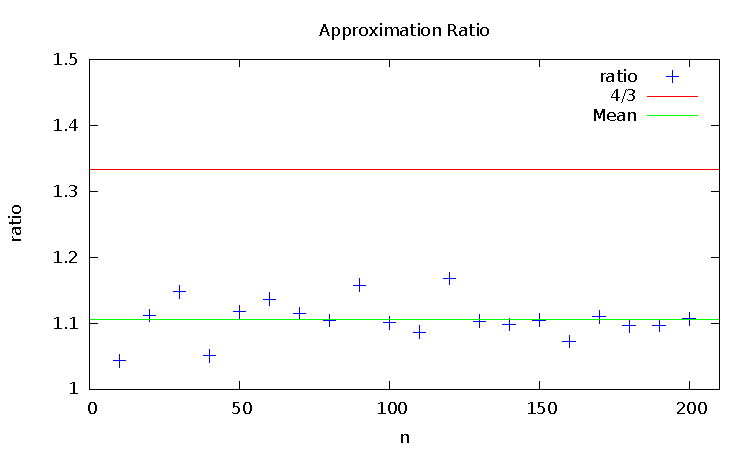
\includegraphics[width=0.5\textwidth]{plot1.pdf}
\end{center}
As observed in the plot, none of the points exceed the 4/3-line. Actually the majority of the points linger between the 1.1 and 1.2 ratio, which is quite good compared to the upper bound. 